\section{x86 Data Movement} 

  \begin{definition}[Data Types]
    In x86, 
    \begin{enumerate}
      \item A \textbf{word} refers to 
    \end{enumerate}
  \end{definition}

\subsection{Registers}

  The specific type of registers that are available to a CPU depends on the computer architecture, or more specifically, the ISA, but here is a list of common ones for the x86-64. We have \texttt{\%rax}, \texttt{\%rbx}, \texttt{\%rcx}, \texttt{\%rdx}, \texttt{\%rsi}, \texttt{\%rdi}, \texttt{\%rbp}, \texttt{\%rsp}, \texttt{\%r8}, \texttt{\%r9}, \texttt{\%r10}, \texttt{\%r11}, \texttt{\%r12}, \texttt{\%r13}, \texttt{\%r14}, \texttt{\%r15}. Therefore, the x86-64 Intel CPU has a total of 16 registers for storing 64 bit data. However, it is important to know which registers are used for what. 

  \begin{definition}[Parameter Registers]
    Compilers typically store the first six parameters of a function in registers 
    \begin{equation}
      \texttt{\%rdi}, \texttt{\%rsi}, \texttt{\%rdx}, \texttt{\%rcx}, \texttt{\%r8}, \texttt{\%r9}, 
    \end{equation}
    respectively. 
  \end{definition}

  \begin{definition}[Return Register]
    The return value of a function is stored in the 
    \begin{equation}
      \texttt{\%rax} 
    \end{equation}
    register.
  \end{definition}

  \begin{definition}[Stack and Frame Pointers]
    The \texttt{\%rsp} register is the \textbf{stack pointer}, which points to the top of the stack. The \texttt{\%rbp} register is the \textbf{frame pointer}, or \textbf{base pointer}, which points to the base of the current stack frame. In a typical function prologue, \textbf{\%rbp} is set to the current stack pointer (\textbf{\%rsp}) value, and then \texttt{\%rsp} is adjusted to allocate space for the local variables of the function. This establishes a fixed point of reference (\texttt{\%rbp}) for accessing those variables and parameters, even as the stack pointer (\texttt{\%rbp}) moves.
  \end{definition}

  \begin{definition}[Instruction Pointer]
    The \texttt{\%rip} register is the \textbf{instruction pointer}, which points to the next instruction to be executed. Unlike all the registers that we have shown so far, programs cannot write directly to \texttt{\%rip}. 
  \end{definition}

  \begin{definition}[Notation for Accessing Lower Bytes of Registers]
    Sometimes, we need a more fine grained control of these registers, and x86-64 provides a way to access the lower bits of the 64 bit registers. We can visualize them with the diagram below. 
    \begin{figure}[H]
      \centering 
      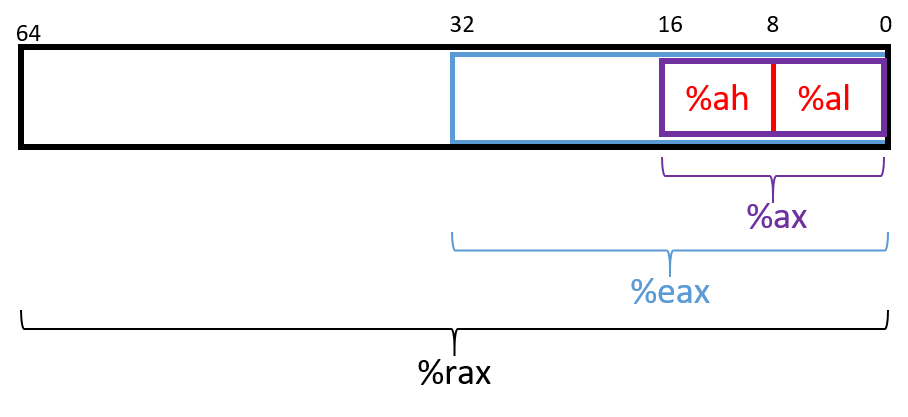
\includegraphics[scale=0.6]{img/register_subsets.png}
      \caption{The names that refer to subsets of register \texttt{\%rax}.} 
      \label{fig:register_subsets}
    \end{figure}
    A complete list is shown below. 
    \begin{table}[H]
      \centering
      \begin{tabular}{|l|l|l|l|}
      \hline
      \textbf{64-bit Register} & \textbf{32-bit Register} & \textbf{Lower 16 Bits} & \textbf{Lower 8 Bits} \\ \hline
      \%rax & \%eax & \%ax & \%al \\ \hline
      \%rbx & \%ebx & \%bx & \%bl \\ \hline
      \%rcx & \%ecx & \%cx & \%cl \\ \hline
      \%rdx & \%edx & \%dx & \%dl \\ \hline
      \%rdi & \%edi & \%di & \%dil \\ \hline
      \%rsi & \%esi & \%si & \%sil \\ \hline
      \%rsp & \%esp & \%sp & \%spl \\ \hline
      \%rbp & \%ebp & \%bp & \%bpl \\ \hline
      \%r8 & \%r8d & \%r8w & \%r8b \\ \hline
      \%r9 & \%r9d & \%r9w & \%r9b \\ \hline
      \%r10 & \%r10d & \%r10w & \%r10b \\ \hline
      \%r11 & \%r11d & \%r11w & \%r11b \\ \hline
      \%r12 & \%r12d & \%r12w & \%r12b \\ \hline
      \%r13 & \%r13d & \%r13w & \%r13b \\ \hline
      \%r14 & \%r14d & \%r14w & \%r14b \\ \hline
      \%r15 & \%r15d & \%r15w & \%r15b \\ \hline
      \end{tabular}
      \caption{Register mapping in x86-64 architecture}
      \label{table:register_mapping}
    \end{table}
  \end{definition}

\subsection{Addressing Modes}

  \begin{example}[Immediate Addressing]
    \begin{lstlisting} 
      movq $0x4, %rax
    \end{lstlisting}
  \end{example}

  \begin{example}[Normal Addressing]
    The following example shows the source operand being a memory address, with normal addressing, and the destination operand being a register.  
    \begin{lstlisting} 
      movq (%rax), %rbx
    \end{lstlisting}
  \end{example}

  \begin{example}[Displacement Addressing]
    The following example shows the source operand being a memory address and the destination operand being a register. They are both addressed normally. 
    \begin{lstlisting} 
      movq 8(%rdi), %rdx
    \end{lstlisting}
  \end{example}

  \begin{example}[Indexed Addressing]
    The following shows the source operand being a memory address and the destination operand being a register. Say that \texttt{\%rdx = 0xf000} and \texttt{\%rcx = 0x0100}. Then 
    \begin{equation}
      \texttt{0x80(,\%rdx,2) = Mem[2*0xF000 + 0x80] = Mem[0x1E080]}
    \end{equation}
    We see that 
    \begin{lstlisting} 
      movq 0x100(%rdi, %rsi, 8), %rdx
    \end{lstlisting}
  \end{example}

